\documentclass{article}
\usepackage[utf8]{inputenc}
\usepackage{placeins}
\usepackage{caption}        % better captions
\usepackage{subcaption}     % for subfigures
\title{OpenMP:Course}
\author{Oliver Siig, Sudarshan Vijay}
\date{19th of January 2020}

\usepackage{natbib}
\usepackage{graphicx}

\begin{document}

\maketitle

\section{Introduction}
For this project we have implemented an iterative numerical solution to the Poisson equation:
\begin{equation}
\frac{\partial^2u}{\partial x^2}+\frac{\partial^2u}{\partial y^2}=-f(x,y),\hspace{2cm}(x,y)\in \Omega
\end{equation}
Where $u=u(x,y)$ is a function we wish to find, $f(x,y)$ is a source term and $\Omega$ defines the domain, in this case $\{|x|,|y|\}\leq 1$. The problem we consider is the heat distribution in a room described by the source term $f(x,y)=200$ for $0\leq x\leq 1/3; -2/3\leq y \leq -1/3$ and 0 in the rest of the domain. The boundaries of the domain are given as $u(x,1)=u(1,y)=u(-1,y)=0; u(x,-1)=0$. As an initial guess, we have set $u(x,y)=0$ for all other values of $x$ and $y$ within the domain.\\

The problem has been solved using two distinct iterative methods; the \emph{Jacobi method} and the \emph{Gauss-Seidel method}. They both iterate over a discretized representation of the problem given as a $N\times N$ grid. using a finite-difference method. They differ in their approach to the problem however, as the former operates on the full grid at different time steps, while the latter includes updated adjacent points calculated at a given time step when calculating the next point on the grid. The problem was considered solved once the grid had reach a convergence criteria, given as a maximum difference in the sum of the absolute values of all points of the grid, i.e. the norm of the matrix. 
\subsection{Comparison of Gauss-Seidel and Jacobi}

We have computed the number of iterations required for both algorithms to converge for a number of grid sizes, the results are illustrated in Figure \ref{fig:question2}. We notice that there is a clear trend in convergence, irrespective of problem size and that the Gauss-Seidel algorithm converges almost twice as fast as the Jacobi iteration method. These results are in good agreement with the behavior expected of the two algorithms, as the latter is constantly updating the grid and using the most recent estimate of the function value.\\

\begin{figure}
    \centering
    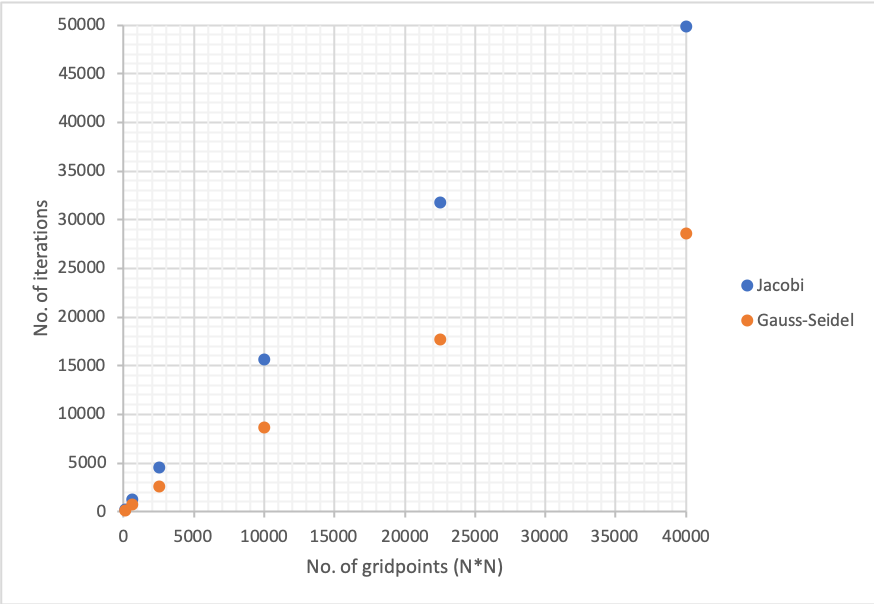
\includegraphics[width=8cm]{figures/question2.png}
    \caption{Number of iterations for GS and Jacobi iterations to converge plotted against the size of the matrix}
    \label{fig:question2}
\end{figure}
In addition to the number of iterations required for the grids to converge, we have also computed the number of grid point updates per second, by varying the no. of time steps, $k$, on a 200x200 grid and measuring the total computation time. While this time does include other operations, it gives an accurate representation of the total run time of each algorithm. As any implementation would require a data transfer between time steps in the Jacobi method, it was expected that the continuously-updating Gauss-Seidel method would perform better here as well.\\

\begin{figure}[!h]
    \centering
    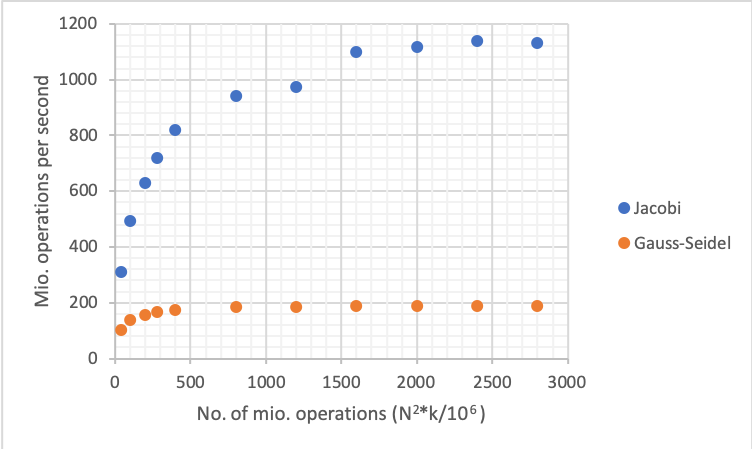
\includegraphics[width=8cm]{figures/question2b.png}
    \caption{Number of iterations for GS and Jacobi iterations to converge plotted against the size of the matrix}
    \label{fig:question2b}
\end{figure}
Surprisingly, the exact opposite trend is seen in Figure \ref{fig:question2b}, with the Jacobi method outperforming the Gauss-Seidel by a large margin. The source of this is not clear, but the results could indicate that the Gauss-Seidel has not been written as efficiently as the Jacobi algorithm. The total computation time includes a number of different operations, including the norm calculations which can have influenced the results. Furthermore, the analysis might have yielded different results, if the test had been performed by updating $N$ rather than $k$. As the remainder of this report is concerned with the implementation of a parallel version of the Jacobi method, the lacking efficiency of the Gauss-Seidel method has not been explored further.

\section{OpenMPI Jacobi}

The simplest implementation of our OpenMP code was to add an OMP statement in the outermost loop. Subsequent attempts are described below. 

A DO WHILE loop was used to test for convergence or fail conditions. This reduced the need to use IF statements which needed OMP single comments. 
\begin{verbatim}
    DO WHILE ( k .LT. k_max .AND. ABS(norm_diff) .GT. 1D-10 )
\end{verbatim}

All arithmetic operations were performed within the same DO loop. The two shown here are change in NEW to OLD matrices for each element of the Jacobi iteration. The norm is also calculated within the same DO loop. 

\begin{verbatim}
 47         !$OMP DO private(i,j) &
 48         !$OMP reduction(+:norm_new) &
 49         !$OMP reduction(+:norm_old)
 50         ! $OMP shared(N,grid_spacing,OLD,NEW,SOURCE)
 51         DO j=2,N-1 ! Inner iterator last
 52           DO i=2,N-1
 53             NEW(i,j) = (1./4.) * ( OLD(i-1,j) + OLD(i+1,j) &
 54                                  + OLD(i,j-1) + OLD(i,j+1) &
 55                                  + ( grid_spacing**2 ) * SOURCE(i,j) )
 56             norm_old = norm_old + OLD(i,j)**2
 57             norm_new = norm_new + NEW(i,j)**2
 58
 59           END DO
 60         END DO
 
\end{verbatim}

\FloatBarrier

 \subsection{Scaling with Amdahls law}
 
 Scaling was tested based on the number of cores used. The rate of increase deteriorated after 2 cores as shown in Figure \ref{fig:scaling_opt}
 \clearpage
 \begin{figure}
     \centering
     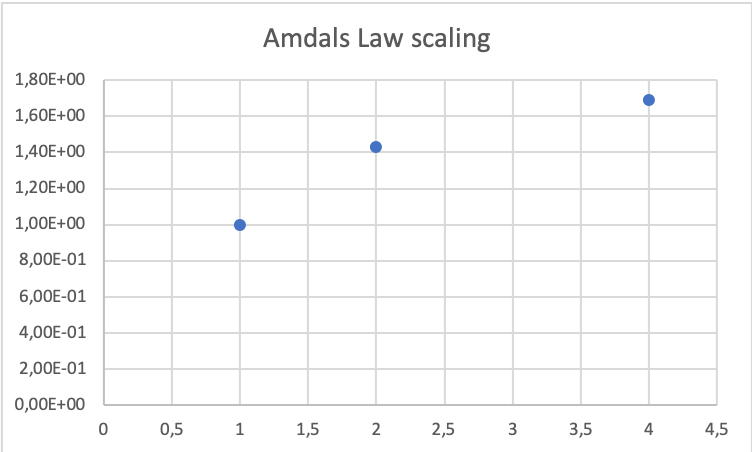
\includegraphics[width=8cm]{figures/scaling_opt.png}
     \caption{Scaling of Optimised code}
     \label{fig:scaling_opt}
 \end{figure}
\subsection{Comparison with Mandelbrot}
As an additional benchmark of the OpenMPI Jacobi we have compared the code to a previously implementation of a solution to the well-known Mandelbrot fractal. Simulations for varying values of k. As the Mandelbrot does not always run to 'count max', it was chosen to set $count\_max=2k\max$, estimating that Mandelbrot runs through roughly half of the possible counts, to get results within the same order of magnitude. As Figure \ref{fig:mandel} shows, the Mandelbrot program scales significantly better than the Jacobi program, particularly when going from 2 to 4 cores. Additionally, both codes seem to exhibit the same scaling behavior regardless of the k-value chosen, at least within this interval. This is in line with expectations, as the Jacobi program contains several code parts, some of which require exclusively using one worker (using an 'OMP SINGLE' statement.
\clearpage
\begin{figure}[h]
\centering
\begin{subfigure}{.49\textwidth}
  \centering
  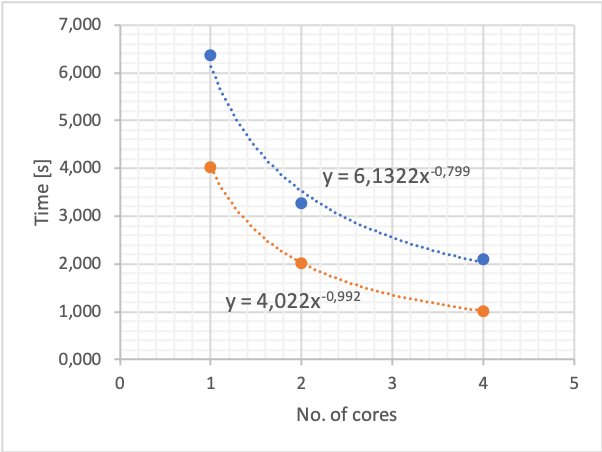
\includegraphics[width=1\linewidth]{k1000.png}
  \caption{k=1000}
  \label{fig:foursub1}
\end{subfigure}%
\begin{subfigure}{.49\textwidth}
  \centering
  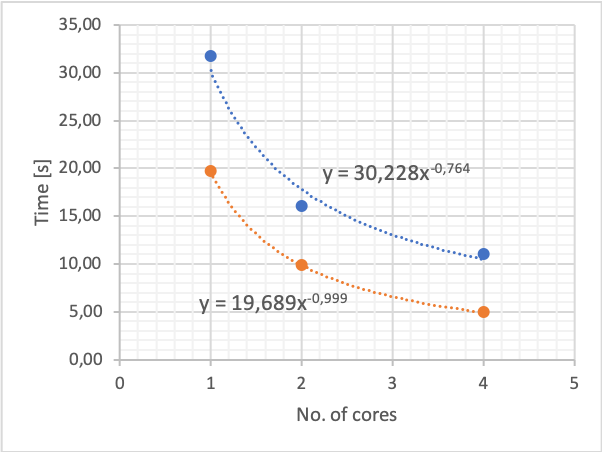
\includegraphics[width=1\linewidth]{k5000.png}
  \caption{k=5000}
  \label{fig:foursub2}
\end{subfigure}
\begin{subfigure}{.49\textwidth}
  \centering
  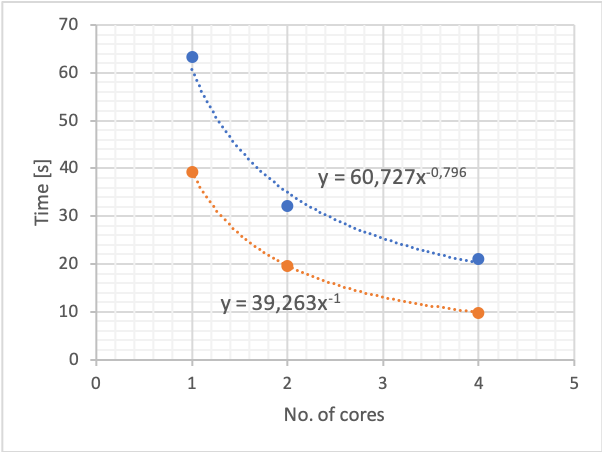
\includegraphics[width=1\linewidth]{k10000.png}
  \caption{k=10000}
  \label{fig:foursub3}
\end{subfigure}
\begin{subfigure}{.49\textwidth}
  \centering
  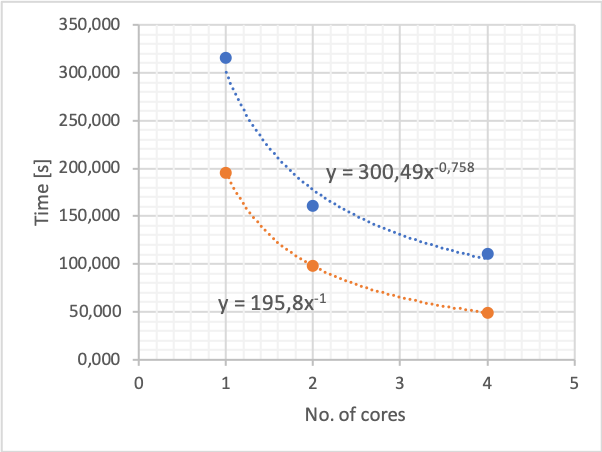
\includegraphics[width=1\linewidth]{k50000.png}
  \caption{k=50000}
  \label{fig:foursub4}
\end{subfigure}
\caption{Scaling of the Jacobi (orange) vs Mandelbrot (blue) programs using 1, 2 and 4 cores and varying k-values. All of the mandelbrot runs scale almost perfectly as 1/x, while the scaling for the Jacobi is worse, particularly from 2 to 4 cores.}
\label{fig:mandel}
\end{figure}
\section{Making an OpenMP Gauss-Seidel}
While there are obvious advantages of the Gauss-Seidel over the Jacobi method, as convergence takes fewer step and \emph{should} be faster to iterate over, implementing a parallel version is significantly more challenging, as the order of operations is crucial in a continuously updating model. In essence, the model cannot be parallelized over columns nor rows, as a given point requires information from both the previous row and column for any given time step. If one was to parallelize the Gauss-Seidel method one would have to account for this, which could be done in a number of ways. One possibility would be to run through the grid along a diagonal perpendicular to $i=j$, i.e. implementing a condition $i<j$ when going through a column. This code could be parallelized to a varying, from being sequential at $(0,0)$ and $(N,N)$ to N parallel updates along the $\{(N,0),(N-1,1),...,(1,N-1),(0,N)$ diagonal. This would naturally have to be adapted for the specific parallel architecture; a distributed memory method has been proposed to acheive this \cite{SHANG20091369}.
\bibliographystyle{plain}
\bibliography{references}
\end{document}
